\chapter{Prerequisites}\label{chap:prerequisites}

In this chapter, we briefly review some of the more fundamental concepts on which the rest of this work is built. Section~\ref{sec:band-theory} covers some essentials of condensed matter physics, to the degree that is necessary here; in particular, some of the key assumptions underlying our description are highlighted, and the significance of the Brillouin zone and the Berry phase are explained. Section~\ref{sec:homology-cohomology} provides the necessary mathematical background; in particular, the topological tools of homology and cohomology are treated. Readers who are at least somewhat familiar with the concepts in either section are free to skip over them, and refer back to their contents later as needed.

\markedsection{Condensed matter}{Concepts in condensed matter}\label{sec:band-theory}

We offer here a brief review of the physics of electronic materials, to the extent that is relied on in this thesis. The concepts set out here are explored in great generality in standard reference works such as Ref.~\cite{AshcroftMermin_bands}, but we will only require a select few specialised details.

The electronic transport properties of materials can be understood in terms of the energy levels that the electronic states that inhabit them may occupy, in close analogy to the electronic orbitals in a single atom; in a material, these levels are referred to as \emph{energy bands}. In the ground state of a material, the Pauli exclusion principle ensures that the energy bands are occupied up to a certain level, known as the Fermi energy. The manner in which electricity is (or is not) conducted in a system is then determined by the way in which the bands are organised around the Fermi energy; this is illustrated in Figure~\ref{fig:bands}.
\begin{figure}[htb!]
	\centering
	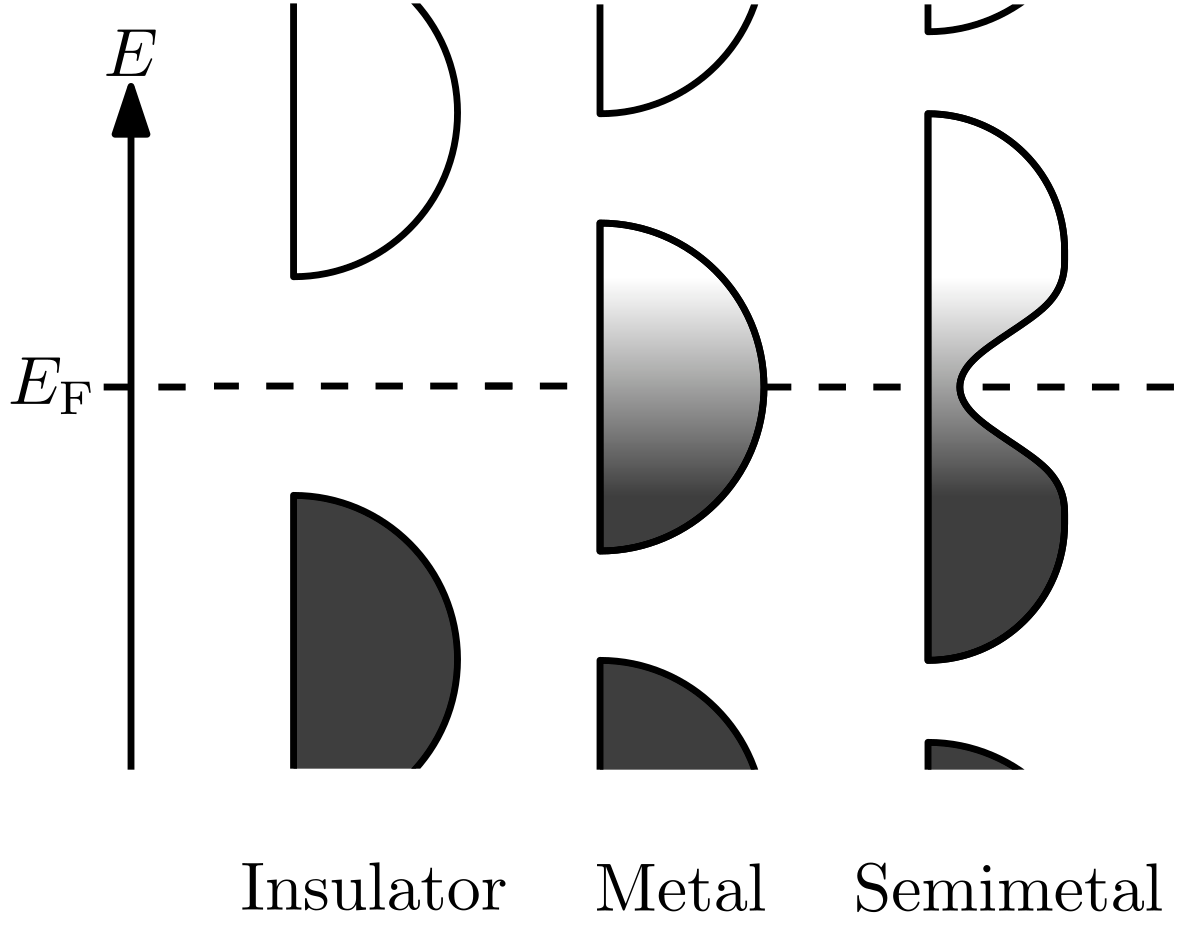
\includegraphics[width=.7\linewidth]{Images/bands}
	\caption{Schematic illustration of the energy bands related to different types of materials. Occupied states are indicated in grey, while unoccupied states are white. In an insulator, the Fermi energy lies between a fully occupied valence band and a fully empty conduction band. On the other hand, metals and semimetals are characterised by bands which overlap or touch at the Fermi energy, respectively. The colour gradient across the Fermi energy $E_F$ indicates that the system is not in the ground state, and the electrons in these states are mobile.}
	\label{fig:bands}
\end{figure}
In general, partially occupied bands give rise to mobile electron states at the Fermi energy, allowing for conduction. This is closely related to the microscopic picture in which the partially occupied outer electron orbits in metal atoms allow mutual exchange of electrons. Here, we will use the common convention of setting the Fermi energy to $E_F=0$.


\subsection{Core assumptions}

We follow three commonly made assumptions in this work in order to make the energy band description mathematically tractable. The first is that the atomic orbitals in the material do not overlap significantly between atomic sites. This is known as the \emph{tight-binding approximation}, and it ensures that the bands exist at discrete energy levels, without being split into different ranges of energies.

The second assumption we make is that the physical properties of the systems under consideration are well approximated by just two energy bands. This is often the case in insulators and semimetals, where the Fermi energy lies between two bands: in this case, the highest occupied band is called the \emph{valence band} and the lowest empty band is the \emph{conduction band}.

The two-band tight-binding model allows for the system to be described by a $2\times2$ Hamiltonian operator. In momentum space, a $2\times2$ Hermitian operator takes on the generic form
\begin{equation}\label{eq:Hamiltonian}
	\Hc(\k) = h_0(\k)\Id + \h(\k)\cdot\bm{\upsigma},
\end{equation}
where $\bm{\upsigma} = (\sigma_x,\sigma_y,\sigma_z)\tran$ is the vector of Pauli matrices, and the number of components in $\k$ depends on the dimensionality of the material. In practice, the trace term parametrised by $h_0$ turns out to not affect the topology of the bands, and as such we will often assume $h_0(\k)=0$.

The actual energy bands are now the eigenvalues of this Hamiltonian,
\begin{equation*}
	E(\k) = h_0(\k) \pm \abs{\h(\k)} = h_0(\k) \pm \sqrt{h_1^2(\k) + h_2^2(\k) + h_3^2(\k)}.
\end{equation*}
It follows that the two bands only touch when $\h(\k) = 0$. Under the assumption that $h_0(\k) = 0$, this means that the system is insulating whenever $\h(\k)$ is non-zero.

The final key assumption that we adhere to is that the materials under consideration are crystalline, i.e. that they are described by a periodic lattice. In this context, a result known as \emph{Bloch's theorem} applies \cite{Bloch_theorem}, which tells us that the real-space eigenstates $\psi(\vb{r})$ of any Hamiltonian can be expressed in terms of plane waves and periodic functions:
\begin{equation*}
	\psi(\vb{r}) = \e^{i\k\cdot\vb{r}} u(\vb{r}),
\end{equation*}
where $u(\vb{r})$ respects the periodicity of the lattice. Consequently, different momenta $\k$ can describe the same eigenstate $\psi(\vb{r})$, as long as the resulting values of $\k\cdot\vb{r}$ differ by a multiple of $2\pi$. As a result, there is a bounded region of momentum space containing only momenta which correspond to distinct eigenstates $\psi(\vb{r})$. This region is referred to as the \emph{Brillouin zone}, and it is precisely the unit cell of the reciprocal lattice; see Figure~\ref{fig:Brillouin_zone}.
\begin{figure}[htb!]
	\centering
	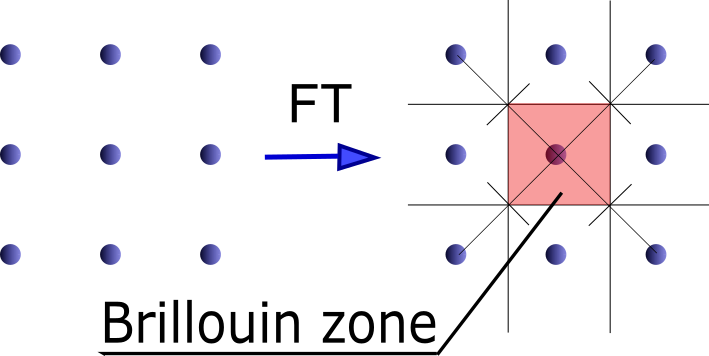
\includegraphics[width=.7\linewidth]{Images/Brillouin_zone}
	\caption{Figure by Gang65, licensed under CC BY-SA 3.0. The Fourier transform of a real-space crystal lattice (left) is a reciprocal lattice in momentum space (right). The Brillouin zone is the unit cell of this reciprocal lattice.}
	\label{fig:Brillouin_zone}
\end{figure}

The boundaries of the Brillouin zone contain momenta which are separated by exactly one unit cell, and these momenta need to be identified with each other to obtain a completely unambiguous description. In $d$ dimensions, the reciprocal lattice is periodic in $d$ directions, so that these boundary identifications give the Brillouin zone the topology of the $d$-dimensional torus $\T^d = \big(S^1\big)^d$; see Figure~\ref{fig:torus}.
\begin{figure}[htb!]
	\centering
	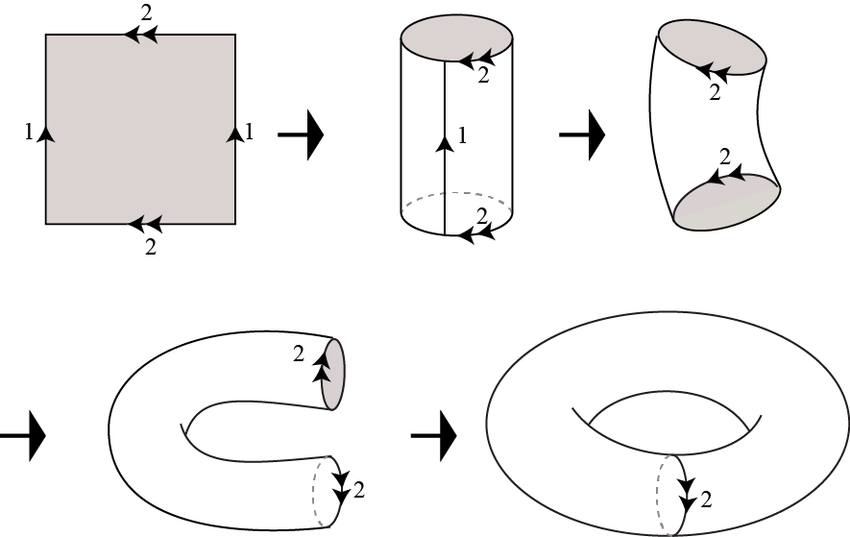
\includegraphics[width=.7\linewidth]{Images/torus}
	\caption{Figure from Ref.~\cite{Potoczak_torus}. The square on the top left represents a two-dimensional Brillouin zone, with the necessary boundary identifications indicated by numbered arrows. This identification is topologically equivalent to ``gluing'' the boundaries together, which gives rise to the 2-torus $\T^2 = S^1\times S^1$.}
	\label{fig:torus}
\end{figure}
Therefore, the Hamiltonian in Equation~\eqref{eq:Hamiltonian} can be considered a function on the torus in this setting; in particular, the vector $\h(\k)$ becomes a map $\h: \T^d\to\R^3$.


\subsection{Berry phase}\label{sec:Berry}

One of the most fundamental concepts in the theory of topological matter is that of the Berry phase \cite{Berry_phase}. The underlying idea is that each electronic eigenstate $\psi(\k)$ of the Hamiltonian carries a complex phase $\phi$ in the electromagnetic gauge group $\U(1)$ (i.e.\ the complex unit circle).\footnote{
Formally, $\phi$ depends on the $\U(1)$ gauge used, but the relative phase change discussed later does not suffer this problem.}
This phase may change as the state $\psi(\k)$ is parallel transported across momentum space; see Figure~\ref{fig:parallel_transport}.
\begin{figure}[htb!]
	\centering
	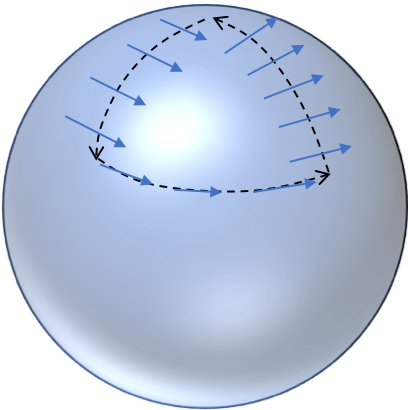
\includegraphics[width=.4\linewidth]{Images/parallel_transport}
	\caption{Figure from Ref.~\cite{Natelson_Berry}. Schematic illustration of parallel transport. The complex phase $\phi$ of a state is represented by the blue arrows. As the state is transported along a closed loop, the phase is kept locally constant, but a non-zero Berry curvature (represented here by the curvature of a sphere) results in a net phase change.}
	\label{fig:parallel_transport}
\end{figure}

The notion of parallel transport is perhaps most familiar in the context of general relativity: there, four-vectors may be transported across spacetime using the Levi--Civita connection. Depending on the Riemann curvature of the intervening spacetime, the orientation of a vector may change as it is transported along a closed loop. The situation is similar for the $\U(1)$ phase of electronic states: the so-called \emph{Berry connection} can be defined as the differential 1-form
\begin{equation*}
	\Ac = A_\mu \dd{k^\mu} = i\bra{\psi(\k)}\partial_\mu\ket{\psi(\k)}.
\end{equation*}
Parallel transport along a line $l\subset\T^d$ in the Brillouin zone is then given by integration of this 1-form, and it induces a change of phase:
\begin{equation*}
	\Delta\phi = \int_l \Ac.
\end{equation*}
This change of phase is exactly what is known as the Berry phase.

Just as the Levi--Civita connection gives rise to Riemann curvature, there is also a \emph{Berry curvature} associated with the Berry connection. This curvature is the differential 2-form given by the exterior derivative of the connection,\footnote{
	To be precise, the Berry curvature is \emph{locally} defined as the exterior derivative, but $\Ac$ may need to be defined in multiple gauges to obtain the full curvature.}
\begin{equation*}
	\Fc = \dd{\Ac} = \big(\partial_\mu A_\nu - \partial_\nu A_\mu\big) \dd{k^\mu}\dd{k^\nu}.
\end{equation*}
This curvature 2-form can be integrated over any two-dimensional subspace $S\subset\T^d$ of the Brillouin zone, and by Stokes' theorem, the result is a measure of the phase change around the boundary of $S$:
\begin{equation*}
	\int_S \Fc = \int_S \dd{\Ac} = \oint_{\dee S} \Ac.
\end{equation*}
This phase change along closed loops needs to be an integer multiple of $2\pi$ to ensure that the electronic states are defined consistently. This puts topological constraints on the Berry curvature, allowing it to be used to study the topology of the system.


\section{Homology and cohomology}\label{sec:homology-cohomology}

The concepts of homology and its dual counterpart cohomology are indispensable tools in the mathematical field of algebraic topology. While seemingly abstract from a physics point of view, many fundamental elements of the physicist's toolbox---such as Stokes' theorem---are formulated most naturally in the context of this theory. Additionally, there are deep results relating the cohomology of a space to the classification of different types of vector bundles over this space. Physically, this relates closely to the classification of topological phases of matter to which this work is dedicated.

Here, we offer a brief introduction to these concepts, aimed at the uninitiated physicist. The goal is not to be completely rigorous, but to give a sufficiently comprehensive understanding that the applications discussed in later chapters may be understood in their proper context. For a more complete picture, the interested reader is referred to standard texts in algebraic topology such as Refs.~\cite{Hatcher_algebraic-topology} and \cite{Bredon_topo-geometry}. A more geometric treatment relying on differential forms is also found in Ref.~\cite{Bott-Tu_differential-forms}.

The basic idea underlying homology is that information about the topology of a space $M$ can be gained from studying non-trivial subspaces of $M$ of various dimensions. Perhaps the simplest conceptual realisation of this idea exists in the closely related \emph{homotopy} theory. In this theory, one defines the $n$th homotopy group $\pi_n(M)$ in terms of maps from the $n$-dimensional sphere $S^n$ into $M$. For example, the first homotopy group $\pi_1(M)$ (also known as the \emph{fundamental group}) records the topologically different ways in which loops $\gamma:S^1\to M$ can sit inside $M$. If two such loops cannot be transformed continuously into each other, then they represent different elements of $\pi_1(M)$.\footnote{
	These deformations may include self-intersections. In particular, this means that different knots (i.e.\ embeddings of $S^1$ in $\R^3$ cannot be distinguished by homotopy. In this context, one needs to use a form of \emph{isotopy} instead, which does not allow self intersections as maps are deformed into each other.}
This fundamental group forms the conceptual basis behind some topological invariants in physics as well, such as that of the Su--Schrieffer--Heeger model discussed in Section~\ref{sec:SSH}.

Despite their conceptual simplicity, homotopy groups can be rather unwieldy in practice: they are generally difficult to compute and may have unpredictable structures. For example, even maps from $S^n$ to a lower-dimensional $S^m$ with $m<n$ may be non-trivial, and calculating the associated higher homotopy groups $\pi_n(S^m)$ of the spheres is an important open problem in algebraic topology.

This is where the closely related homology enters the stage. It is conceptually somewhat more involved than homotopy, and strictly speaking it contains less information. However, there is a great payoff: homology groups are generally much easier to compute and structurally simpler than their homotopy counterparts. Moreover, homology can be dualised into cohomology, which is a construction which is both mathematically and physically very natural.


\subsection{Homology}

The basic building blocks of homology theory are oriented subspaces of a space $M$.\footnote{
	There are different ways of formally defining these oriented subspaces, such as mapping simplices (the $n$-dimensional analogue of triangles) into $M$ or defining a so-called \emph{cell structure} on $M$. Importantly, these different constructions usually give rise to the same homology groups. Therefore, we will be agnostic to the details and focus on the conceptual basis instead.}
Some such subspaces are illustrated for the two-dimensional torus in Figure~\ref{fig:homology-chains}.
\begin{figure}[htb!]
	\centering
	\def\svgwidth{.6\linewidth}
	\import{Images}{homology-chains.pdf_tex}
	\caption{The two-torus $\T^2$. Some of the oriented subspaces that make up chains in the homology theory are highlighted: components of 0, 1, and 2-chains are coloured blue, red and orange, respectively. The orientation of the 0D and 2D subspaces can be canonically induced from an orientation on the torus in this case.}
	\label{fig:homology-chains}
\end{figure}
Topological information can be gained from these subspaces by studying their (oriented) boundaries. The goal of homology is to find subspaces such as $d$ and $e$ in Figure~\ref{fig:homology-chains}, which do not have a boundary, but cannot themselves be written as the boundary of another subset either---unlike $c$, for instance, which is the boundary of $S$. Spaces like $d$ and $e$ detect topological features of the space, such as the hole in the centre of the torus.

To properly define oriented boundaries, we must work in the context of so-called $n$-\emph{chains}, which are linear combinations of $n$-dimensional subspaces of $M$. For example, $a+b$ is a 1-chain on the torus in Figure~\ref{fig:homology-chains}, as is $3a-2c$. Using $n$-chains makes boundaries well-behaved under addition. For example, we may define the boundary of $a$ as the 0-chain $\dee a = p - q$, and similarly $\dee b = q - r$; adding these up, we obtain
\begin{equation*}
	\dee a + \dee b = (p - q) + (q - r) = p - r,
\end{equation*}
which is precisely the boundary of the 1-chain $a+b$.

Formally, an $n$-chain takes the form
\begin{equation*}
	\sum_i c_i X_i,
\end{equation*}
where $X_i\subset M$ are oriented $n$-dimensional subsets of $M$. The coefficients $c_i$ are usually taken to be integers in $\Z$, but they may also be e.g.\ real numbers, rationals or elements of $\Z_2$; to be precise, they must be elements of any fixed Abelian group $G$, which is called the \emph{coefficient group}. A powerful result called the universal coefficient theorem implies that taking coefficients in the integers $G=\Z$ always results in the richest possible homology theory \parencite[\S3.A]{Hatcher_algebraic-topology}; this is why the coefficients are usually assumed to be elements of $\Z$ unless explicitly stated otherwise.

The $n$-chains on $M$ naturally form a group under addition in the coefficient group $G$, which we notate $C_n(M;G)$---or simply $C_n(M)$ when $G=\Z$. The inverses in this group act to invert the orientation of a chain: for example, the chain $-c$ on the pictured torus looks like $c$ with the arrow pointing in the opposite direction.

The boundary of an $n$-chain is always an $(n-1)$-chain. This is even true for $n=0$; points have no boundary, so their boundary is the empty ``$(-1)$-chain'' in $C_{-1}(M;G) = 0$. This means taking the boundary defines\footnote{
	The precise definition of the boundary map depends on the way subspaces are defined, but the properties we discuss here are universal.}
a map $\dee_n$ from $C_n(M;G)$ to $C_{n-1}(M;G)$ for every integer $n$. These maps are group homomorphisms---that is, for integer or real coefficients, they are linear: for instance, we have already seen that $\dee(a+b) = \dee a + \dee b$ on the torus.

The boundary maps $\dee_n$ can be used to arrange the chain groups in a so-called \emph{chain complex}:
\begin{equation*}
	0 \overset{\dee_0}{\leftarrow} C_0(M;G) \overset{\dee_1}{\leftarrow} C_1(M;G) \overset{\dee_2}{\leftarrow} C_2(M;G) \overset{\dee_3}{\leftarrow} \cdots.
\end{equation*}
These chain complexes are usually finite: for example, the 2-torus in Figure~\ref{fig:homology-chains} has no 3-dimensional subspaces, so its chain complex (with integer coefficients) reads
\begin{equation*}
	0 \overset{\dee_0}{\leftarrow} C_0(\T^2) \overset{\dee_1}{\leftarrow} C_1(\T^2) \overset{\dee_2}{\leftarrow} C_2(\T^2) \overset{\dee_3}{\leftarrow} 0.
\end{equation*}
In practice, the subscript on the maps $\dee_n$ is often dropped when talking about specific subspaces.

A very important property of the chain complex is that composing two boundary maps always yields zero; this is often abbreviated as $\dee^2 = 0$. In other words, boundaries have no boundaries. An example of this can be seen in Figure~\ref{fig:homology-chains}: the 1-chain $c$ is the boundary of the 2-chain $S$, but it does not have a boundary itself. In homology terms, chains like $c$ which have no boundaries are called \emph{cycles}. The set of $n$-cycles is denoted $Z_n$ and it forms a subgroup of the $n$-chain group. It is defined in terms of the kernel of $\dee_n$, i.e.\ the $n$-chains that map to the empty chain 0:
\begin{equation*}
	Z_n(M;G) := \ker(\dee_n) \subset C_n(M;G).
\end{equation*}

The property $\dee^2 = 0$ implies that all boundaries are cycles, but crucially, it does not imply the opposite: there may be cycles which are not boundaries. In Figure~\ref{fig:homology-chains}, $d$ and $e$ are such 1-cycles: we cannot find a 2-chain of which $d$ is the boundary, for instance. This implies that the set of $n$-chains which are boundaries is a subgroup of the group of $n$-cycles $Z_n$. The former group is called the group of $n$-\emph{boundaries} and denoted $B_n$. It is defined as the image of $\dee_{n+1}$:
\begin{equation*}
	B_n(M;G) := \im(\dee_{n+1}) \subset Z_n(M;G) \subset C_n(M;G).
\end{equation*}

We can now finally define the homology on $M$. The \emph{$n$th homology group} $H_n$ is the quotient group consisting of all $n$-cycles modulo $n$-boundaries:
\begin{equation*}
	H_n(M;G) := \frac{Z_n(M;G)}{B_n(M;G)} = \ker(\dee_n) / \im(\dee_{n+1}).
\end{equation*}
Again, the coefficient group $G$ is often dropped from the notation under integer coefficients $G=\Z$. The elements of $H_n$ are called \emph{homology classes}, and they are equivalence classes of $n$-cycles. Two $n$-cycles $\gamma_1$ and $\gamma_2$ are called \emph{homologous} if they differ only by a boundary, i.e.\ if $\gamma_1 = \gamma_2 + \dee\Gamma$ for some $n+1$ chain $\Gamma$. In this case they represent the same homology class, and we write $[\gamma_1] = [\gamma_2]\in H_n(M;G)$. For example, the 1-cycle $c$ in Figure~\ref{fig:homology-chains} is the boundary of the 2-chain $S$, and so it is homologous to the empty cycle: $c= 0 + \dee S$, meaning $[c] = 0\in H_1(\T^2)$. Similarly, any $n$-boundary represents the trivial class in $H_n$ in general. Intuitively, this is because a boundary can always be continuously retracted to a point (for example, $c$ can be retracted by shrinking $S$), where it vanishes and becomes the empty cycle.

Another important example of homologous cycles is illustrated in Figure~\ref{fig:homology-classes}.
\begin{figure}[htb!]
	\centering
	\def\svgwidth{.6\linewidth}
	\import{Images}{homology-classes.pdf_tex}
	\caption{The 2-torus $\T^2$, featuring the same 1-cycle $e$ as before, and also a 1-cycle $f$ which is obtained by moving $e$ along the torus. The boundary of the 2-chain $V$ indicated in orange is precisely the difference of these cycles: $\dee V = e - f$. Since $e$ and $f$ differ by a boundary, they are homologous, i.e.\ $[e]=[f]\in H_1(\T^2)$.}
	\label{fig:homology-classes}
\end{figure}
In this case, we see that non-trivial cycles may also represent the same homology class if they can be deformed into each other continuously.

These examples demonstrate an important general property: the homology group classifies cycles that differ from each other topologically, i.e.\ cannot be deformed into one another. As a result, the homology groups $H_n$ have a much simpler structure than the underlying chain groups. For example, the first homology group of the 2-torus $H_1(\T^2)$ consists precisely of elements of the form
\begin{equation*}
	m_d[d] + m_e[e],\quad m_d,m_e\in G=\Z,
\end{equation*}
where $d$ and $e$ are as in Figure~\ref{fig:homology-chains}. It follows that this group looks like two copies of $\Z$:
\begin{equation*}
	H_1(\T^2) \cong \Z^2.
\end{equation*}

The 0th homology group can be obtained by similar logic: all single points on $\T^2$ can be continuously moved to a single point $p$, so that elements of $H_0(\T^2)$ are of the form
\begin{equation*}
	m_p[p],\quad m_p\in\Z,
\end{equation*}
and consequently
\begin{equation*}
	H_0(\T^2) \cong \Z.
\end{equation*}
For similar reasons, if $M$ consists of $k$ connected components, then $H_0(M) = \Z^k$ in general.

Finally, the only two-dimensional subspace of $\T^2$ that represents a non-trivial homology class turns out to be the whole torus itself; as a result, $H_2$ also has a single generator:
\begin{equation*}
	H_2(\T^2) \cong \Z.
\end{equation*}
These three groups completely classify the homology of the 2-torus, since it only admits $n$-chains for $0\leq n\leq 2$. This is a general property of homology: unlike homotopy, where higher homotopy groups may have a highly non-trivial structure, the homology groups $H_n$ of a $d$-dimensional manifold are always 0 for $n>d$ and $n<0$.


\subsection{Cohomology}\label{sec:cohomology}

The chain complex structure underlying homology allows for a natural counterpart called cohomology, which is obtained by \emph{dualising} the chain complex. Dualisation is a concept that shows up all over mathematics; the basic idea is that a mathematical object can be paired with a different object---its \emph{dual}---in order to obtain something like a simple number. A familiar example from physics is that of a covector: in physics notation, any vector $V^\mu$ can be paired with any covector $\omega_\mu$ to obtain a scalar $\omega_\mu V^\mu\in\R$. Formally, a covector is defined as a linear function from the underlying vector space to $\R$.

A similar construction is used to define \emph{cochains} on a manifold $M$. An $n$-cochain is a homomorphism from the $n$-chain group $C_n(M;G)$ into the coefficient group $G$; under the usual integer coefficients, this is a function $C_n(M)\to\Z$ that assigns an integer to each $n$-chain linearly. The cochains form a group which has a very similar structure to the chain group itself. We denote the $n$-cochain group with a raised index:
\begin{equation*}
	C^n(M;G) := \Hom\big(C_n(M;G),G\big).
\end{equation*}

There is an interpretation of cochains with coefficients in $\R$ which is of special relevance to physicists. This comes in the form of integration on differential forms: for example, a 1-form $\Ac$ can be paired with an oriented 1-dimensional subspace $\ell\subset M$ in a line integral, to obtain a real number $\int_{\ell}\Ac\in\R$. The definition of integration can be readily generalised from subspaces of $M$ to chains, so that a differential $n$-form becomes a linear map on the chain group:
\begin{equation*}
	\omega: C_n(M;\R)\to\R,\quad c := \sum_i c_i X_i \mapsto \int_c \omega := \sum_i c_i \int_{X_i}\omega,
\end{equation*}
where as before, $X_i$ are oriented $n$-dimensional subspaces of $M$ and $c_i$ are coefficients in $\R$. This definition of integration gives rise to a complete cohomology theory in terms of differential forms, called \emph{de Rham cohomology}. This theory is fully equivalent to more abstractly defined cohomology with $\R$ coefficient, and offers a useful link to physical observables: the existence of de Rham cohomology means that many topological invariants can be expressed in terms of integrals over differential forms such as the Berry flux 1-form $\Ac$ and the Berry curvature 2-form $\Fc$.

The main shortcoming of de Rham cohomology lies in its real coefficients. As mentioned before, the universal coefficient theorem implies that $\Z$ coefficients may provide richer homology groups, and the same also holds for cohomology. This is especially true when the homology and cohomology groups contain $\Z_2 := \Z/2\Z$ factors (referred to as \emph{torsion}\footnote{
	Formally, torsion also includes more general factors $\Z_k$, but these do not tend to appear in the physics literature as often.}),
corresponding to $\Z_2$ physical invariants; these appear especially often on the non-orientable manifolds studied in this work. These factors disappear under $\R$ coefficients, relating to the fact that $\R/2\R = 0$. Still, many of the associated invariants may be expressed using modified integral formulas, and in any case, the de Rham theory offers a physically intuitive perspective on cohomology. For these reasons, we will continue to use it as an analogy for the more abstract concepts of integer-valued cohomology.

Just as in homology, the cochain groups of cohomology are gathered into a \emph{cochain complex}: for example, the cochain complex of the 2-torus is
\begin{equation*}
	0 \overset{\delta_{-1}}{\rightarrow} C_0(\T^2) \overset{\delta_0}{\rightarrow} C_1(\T^2) \overset{\delta_1}{\rightarrow} C_2(\T^2) \overset{\delta_2}{\rightarrow} 0.
\end{equation*}
The maps $\delta_n: C^n\to C^{n+1}$ are called \emph{coboundary} maps, and they are a natural result of dualising the boundary maps $\dee_{n+1}: C_{n+1}\to C_n$, meaning they are uniquely defined by the property
\begin{equation}\label{eq:boundary-duality}
	\delta\omega(c) = \omega(\dee c).
\end{equation}
This duality takes on a familiar form in de Rham cohomology: there, the coboundary map is the exterior derivative $\dd$ on differential forms, and the duality above becomes
\begin{equation*}
	\int_{c}\dd{\omega} = \int_{\dee c}\omega,
\end{equation*}
which is precisely Stokes' theorem. For example, suppose a Berry connection 1-form $\Ac$ (as defined in Section~\ref{sec:Berry}) exists on the 2-torus in Figure~\ref{fig:homology-chains}. Then the Berry curvature 2-form $\Fc$ can locally be written as $\Fc = \dd{\Ac}$, and Stokes' theorem tells us that
\begin{equation*}
	\int_{S}\Fc = \int_{S}\dd{\Ac} = \int_{\dee S}\Ac = \int_c\Ac.
\end{equation*}
This dual property of the coboundary maps also ensures that the cochain complex inherits the $\dee^2 = 0$ property of the chain complex: for any $n$-cochain $\omega$ and $n+2$-chain $c$, we find
\begin{equation*}
	\delta^2\omega(c) = \omega(\dee^2 c) = \omega(0) = 0,
\end{equation*}
so that there is a similar $\delta^2=0$ property here.

The construction of the cohomology groups from the cochain complex proceeds completely analogously to that of the homology groups. Just as an $n$-cycle is an $n$-chain with no boundary, an $n$-\emph{cocycle} is a cochain $\omega$ which has no coboundary, i.e.\ for which $\delta{\omega} = 0$. In de Rham cohomology, cocycles are called \emph{closed} differential forms (i.e.\ those with $\dd{\omega} = 0$). The $n$-cocycles form a group which is denoted (again using a raised index) as
\begin{equation*}
	Z^n(M;G) := \ker(\delta_n).
\end{equation*}
Similarly, an $n$-\emph{coboundary} is defined as an $n$-cochain $\omega$ which can be written as $\omega=\delta{\eta}$ for some $(n-1)$-cochain $\eta$. In the context of de Rham cohomology, the coboundaries are referred to as \emph{exact} differential forms (i.e.\ forms which can be written as $\omega = \dd\eta$. Again, the $n$-coboundaries form a group which is denoted
\begin{equation*}
	B^n(M;G) := \im(\delta_{n-1}).
\end{equation*}

The $\delta^2 = 0$ property of the cochain complex implies that all coboundaries are cocycles. In de Rham cohomology, this corresponds precisely to the Bianchi identity $\dd^2=0$, which says that all exact forms are closed. As before, this implies that $B^n$ is a subgroup of $Z^n$, and we can define the $n$th \emph{cohomology group} as their quotient:
\begin{equation*}
	H^n(M;G) := \frac{Z^n(M;G)}{B^n(M;G)} = \ker(\delta_n) / \im(\delta_{n-1}).
\end{equation*}
The elements of this group are called \emph{cohomology classes}. In the de Rham picture, non-trivial cohomology classes are represented by forms which are closed, but not exact. For example, this can be the case for the Berry curvature 2-form $\Fc$: while it can always be written as $\dd{\Ac}$ \emph{locally}, this depends on a local choice of gauge. Globally, there may be gauge singularities preventing $\Ac$ from being well defined everywhere. As a result, an expression like $\int_{\T^2}\Fc$ may have a non-zero value, precisely because $\T^2$ itself is a 2-cycle with non-trivial global topology. In this case, $\Fc$ represents a non-zero cohomology class $[\Fc]\in H^2(\T^2;\R)$.

This close link between cohomology classes and non-trivial cycles ensures that the cohomology groups $H^n$ are intimately related to the homology groups $H_n$ in their structure; in fact, in the absence of the aforementioned $\Z_2$ torsion factors, there is a direct isomorphism $H^n(M)\cong H_n(M)$ for every $n\in\Z$.\footnote{
	To be precise, when there are torsion factors in some homology group $H_n$, they will appear ``one dimension up'' in the cohomology group $H^{n+1}$ instead of $H^n$. Incidentally, since there is no torsion in de Rham cohomology, this means that $H^n(M;\R) \cong H_n(M;\R)$ in full generality.}
This means that for instance, the cohomology groups of the 2-torus are the same as the homology groups:
\begin{equation*}
	H^0(\T^2) \cong \Z;\quad H^1(\T^2) \cong \Z^2;\quad H^2(\T^2)\cong \Z.
\end{equation*}
There is a straightforward interpretation of these groups in terms of their homology counterparts: for example, $H^1(\T^2)$ is generated by the cocycles (1-forms) that evaluate to 1 on either of the two non-trivial loops that generate $H_1(\T^2)$, and to 0 on the other.

Finally, we should reiterate what the value in this whole process of dualisation is, given that the cohomology groups are so easily computed from their homology counterparts. The answer is that cohomology, despite being seemingly more involved than homology, is in some ways a more natural theory from both a physical and a mathematical point of view. Physically, the interpretation in terms of differential forms allows topological invariants to be written as integrals of physical quantities. Mathematically, it turns out that there are deep links between cohomology theory and the topological classification of vector bundles; for example, the complex line bundles over a manifold $M$ are always fully classified by $H^2(M)$. These line bundles turn out to be in direct correspondence to certain topological states of matter in a two-band model. The full classification of vector bundles is the subject of an advanced area of mathematics known as K-theory, which is really a generalised cohomology theory. K-theory in turn plays an important role in the more general classification of topological phases of matter \cite{FreedMoore_K-theory,Thiang_K-theory}.